\documentclass{article}
\usepackage{url}
\usepackage{graphicx}
\graphicspath{ {./source/images/} }

\begin{document}

  \section{Event-driven Programming paradigm}
    \subsection{Single thread}
      Single threaded or sequential programming is in which requests are
      processed by a single thread. If the thread is doing some blocking task
      like IO then the program can't handle any other requests until the
      request is processed.

      Example of single threaded server
      \begin{verbatim}
        import time

        from http import server
        from socketserver import ThreadingMixIn


        class RequestHandler(server.SimpleHTTPRequestHandler):

            def do_GET(self):
                start_time = time.time()
                time.sleep(5)
                end_time = time.time()
                self.send_response(200, "OK")
                self.end_headers()
                response = (
                    "Started at {}, Ended at {} difference {}".format(
                        start_time, end_time, end_time - start_time
                    )
                )
                self.wfile.write(response.encode('utf-8'))
                return


        if __name__ == "__main__":
            with server.HTTPServer(
                ('localhost', 8000), RequestHandler
            ) as http_server:
                http_server.serve_forever()
      \end{verbatim}

    \subsection{Multi-Threaded}
      Converting above program to a multithreaded version will help. A
      multithreaded program will handle each HTTP request in a new thread and
      thus it can handle multiple requests at the same time.

      \begin{verbatim}
        import time

        from http import server
        from socketserver import ThreadingMixIn


        class RequestHandler(server.SimpleHTTPRequestHandler):

            def do_GET(self):
                start_time = time.time()
                time.sleep(5)
                end_time = time.time()
                self.send_response(200, "OK")
                self.end_headers()
                response = (
                    "Started at {}, Ended at {} difference {}".format(
                        start_time, end_time, end_time - start_time
                    )
                )
                self.wfile.write(response.encode('utf-8'))
                return

        with server.HTTPServer(
          ('localhost', 8000), RequestHandler
        ) as http_server:
            http_server.serve_forever()
      \end{verbatim}

      Compared to the single threaded approach, a program using  multithreaded
      approach will be able to achieve more performance because a multithreaded
      server will spawn a new thread for each new request. And thus, when the
      thread is blocking, it can handle another request during that time.

      But using this approach will bring another problem. When bunch of new
      requests are coming (usually higher than cores of a processor), then
      blocking thread is actually blocking a CPU core on which it is executing.

      In below section I am comparing a multi-threaded example using Apache
      Benchmark tool.

      \begin{verbatim}
        ab -n 100 -c 100 -s 120 http://localhost:8000
      \end{verbatim}

      Some times Apache Benchmark will require the internet connection even if
      we are testing local services.

      Explaining above command by its arguments, \textbf{-n} is a short-hand
      for number of requests to be fired. \textbf{-c} is a concurrent requests
      the tool will fire at the same time. \textbf{-s} is a short hand for
      total number of seconds after which the tool will timeout a request.

      Any threaded server can handle (total number of cores * 1.5 ) + 1 number
      of requests at one time. The server can't handle more concurrent requests
      at a same time. The server will process those requests in batches.

    \subsection{Event-driven}
      Now, if we convert above example into an event-driven asynchronous code
      then it will look as below.

      \begin{verbatim}
        import time

        from twistedinternet import reactor
        from twistedinternet.task import deferLater
        from twistedweb.resource import Resource
        from twistedweb.server import Site, NOT_DONE_YET


        class BusyPae(Resource):
            isLeaf =True

            def _delyedResponse(self, request):
                end_ime = time.time()
                respnse = "Ended at {}".format(end_time)
                requst.write(response.encode("utf-8"))
                requst.finish()

            def rendr_GET(self, request):
                d = eferLater(reactor, 40, lambda: request)
                d.adCallback(self._delayedResponse)
                retun NOT_DONE_YET


        factory = Sie(BusyPage())
        reactor.listnTCP(8000, factory)
        reactor.run()
      \end{verbatim}

    Now let's measure the performance of this code with the Apache benchmarking
    tool and then compare it with all of our previous results.

    Below is the same command which we had used earlier to compare the
    multi-threaded approach.

    \begin{verbatim}
      ab -n 100 -c 100 -s 120 http://localhost:8000
    \end{verbatim}

    The output statistics of both the command will be different. The
    asynchronous approach will be able to handle all the requests at the same
    time. Reason behind this is when the request is coming, the IO thread is
    trying to process the request. During that time, if it is blocked the code
    is handled by event-driven approach and the thread is again available for
    entertaining another request. The processing of request is again resumed
    when the duration of IO is completed and returned.

    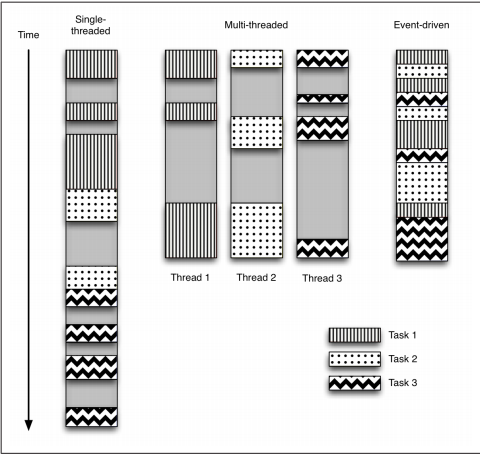
\includegraphics{event_driven_comparision.png}

  \section{Introduction to Twisted programming}

    \subsection{History}
      Twisted was invented by \texttt{Glyph Lefkowitz} in the year October 22,
      2002 which is almost 16 years before. It is an old giant.

    \subsection{Current situation}
      At present, the Twisted framework is developed and managed by its
      community. Latest stable version is \textbf{18.9.x}. The Twisted
      framework is licensed under MIT license. Twisted is based on event-driven
      programming paradigm.

    \subsection{Sockets}
      Twisted programming supports all the TCP, UDP, SSL/TSL based sockets. It
      also supports the Unix sockets.

    \subsection{Protocol}
      Twisted supports many application layer protocols. Such as HTTP, XMPP,
      IMAP, SSH, IRC, FTP and many more.

    \subsection{Applications/Frameworks based on Twisted}

    \begin{itemize}
      \item Buildbot \cite{buildbot}
      \item Omgle video chat service \cite{omegle}
      \item Twilio a cloud telephony provider \cite{twilio}
      \item Twitch.tv a popular Game livestream video sharing \cite{twitch}
      \item Scrapy a framework for scrapping webpages \cite{SCrapy}
    \end{itemize}

    And many more are based on Twisted!

  \section{Echo server and client example}

    \subsection{Echo Server}
      \begin{verbatim}
        from twisted.internet import protocol, reactor


        class EchoServer(protocol.Protocol):

            def dataReceived(self, data):
                print(data)
                self.transport.write(data)


        class EchoFactory(protocol.Factory):

            def buildProtocol(self, addr):
                return EchoServer()


        if __name__ == "__main__":
            reactor.listenTCP(8000, EchoFactory())
            reactor.run()
      \end{verbatim}

      \subsection{Echo client}

      \begin{verbatim}
        from twisted.internet import reactor, protocol


        class EchoClient(protocol.Protocol):

            def connectionMade(self):
                response = "Hello world!"
                self.transport.write(response.encode("utf-8"))

            def dataReceived(self, data):
                print(data)
                self.transport.loseConnection()


        class EchoFactory(protocol.ClientFactory):

            def buildProtocol(self, addr):
                protocol = EchoClient()
                protocol.factory = self
                return protocol

            def clientConnectionFailed(self, connector, reason):
                reactor.stop()

            def clientConnectionLost(self, connector, reason):
                reactor.stop()


        if __name__ == "__main__":
            reactor.connectTCP("localhost", 8000, EchoFactory())
            reactor.run()
      \end{verbatim}

  \section{Reactor}
    Reactor is the core of the event loop. It is responsible for waiting for
    the event and notify the program when the event is occurred. Reactor is
    dependent on platform specific libraries. Twisted will automatically choose
    default platform specific library.

    For under the hood details, In GNU/Linux platform it tries to fetch for
    epoll \cite{epoll}.  If epoll \cite{epoll} is not available, it will use
    poll \cite{poll}. All the POSIX compliant platforms it will use poll. All
    other platforms such as Windows and Macintosh it will use select reactor.

    You have to register your callbacks to the reactor and have to start it.
    Once the reactor is start, it will listen to the events and notifies to the
    program forever or until \texttt{reactor.stop} is called.

    In our echo server and echo client example, below code is representing the
    reactor. The \texttt{reactor.run()} will start the event loop until the
    \texttt{SIGINT} or \texttt{reactor.stop()} is called.

    \begin{verbatim}
      reactor.listenTCP(8000, MyFactory())
      reactor.run()
    \end{verbatim}

  \section{Transport}

    Transport is responsible to provide the behaviour for transferring data to
    the other end of the connection. The transport behaves differently
    according to the connection for example, TCP or UDP will have different
    implementation of transport. 
    In echo client and echo server example below code is representing Transport

    \begin{verbatim}
      self.transport.write()
    \end{verbatim}

    All the transport implementations should be dependent on
    \texttt{ITransport} interface. Below are the common methods of Transport

    \subsection{write} Should write data to the connection.

    \subsection {writeSequence} Should write list of strings to the connection.

    \subsection{loseConnection} Should close the connection after writing
    ending data.

    \subsection{getPeer} Should return remote address of the connection.

  \section{Protocol}
    Protocol will define the behaviour to process the network events in async
    manner. Twisted does have in-built definition for many protocols such as
    HTTP, Telnet, DNS etc. Base class is \texttt{protocol.Protocol}.

    In echo server and echo client example, below code is of Protocol.

    \begin{verbatim}
      \\ Client
      class EchoClient(protocol.Protocol):

          def connectionMade(self):
              request = "Hello, world!"
              self.transport.write(request.encode("utf-8"))

          def dataReceived(self, data):
              print(data)
              self.transport.loseConnection()

      \\ Server
      class EchoServer(protocol.Protocol):

          def dataReceived(self, data):
              print(data)
              self.transport.write(data)
    \end{verbatim}

    All the protocol classes should implement \texttt{IProtocol} interface.
    Common methods are below

    \subsection{makeConnection} Should create a connection.

    \subsection{connectionMade} Should be called when a new connection is made.

    \subsection{dataReceived} Should be called when any data is received from
    the other end of the circuit.

    \subsection{connectionLost} Should be called when the connection is
    terminated.

  \section{Protocol Factory}
    The factory will produce the instance of \texttt{Protocol} when the new
    connection is made. \texttt{Protocol} will be garbage collected when the
    collection is called. The Factory will store configuration details for
    \texttt{Protocol} instances.


    According to our echo server and echo client example, below is the code of
    portable factory.

    \begin{verbatim}
      \\ Server
      class EchoFactory(protocol.Factory):

          def buildProtocol(self, addr):
              return EchoServer()


      \\ Client
      class EchoFactory(protocol.ClientFactory):

          def buildProtocol(self, addr):
              protocol = EchoClient()
              protocol.factory = self
              return protocol

          def clientConnectionFailed(self, connector, reason):
              reactor.stop()

          def clientConnectionLost(self, connector, reason):
              reactor.stop()
    \end{verbatim}

    The factory is following \texttt{IProtocolFactory} interface. There client
    implementation of common factory methods is \texttt{ClientFactory}. Common
    methods are as per below

    \subsection{buildProtocol} should create the instance of Protocol class.

    From the above example, purpose of protocol factories might not be clear in
    your mind. For that reason, we will conver another example.

    \begin{verbatim}
    from twisted.internet.protocol import Factory
    from twisted.protocols.basic import LineReceiver
    from twisted.internet import reactor


    class ChatProtocol(LineReceiver):

        def __init__(self, factory):
            self.factory = factory

        def connectionMade(self):
            self.factory.users.append(self)

        def lineReceived(self, line):
            for user in self.factory.users:
                if user != self:
                    user.transport.write(line + b"\r\n")


    class ChatFactory(Factory):

        def __init__(self):
            self.users = []

        def buildProtocol(self, addr):
            return ChatProtocol(self)


    if __name__ == "__main__":
        reactor.listenTCP(6000, ChatFactory())
        reactor.run()
    \end{verbatim}

    Connect with chat server using multiple connections made by \texttt{telnet}
    program. This will allow to communicate multiple clients as in chatting in
    group. In that code, concurrent client instances are stored at Protocol
    Factory. Whenever you have to store persistent information beyond the
    life cycle of your socket, you should store that in the Protocol Factory.
    Protocol will be created and garbage collected with connection.

  \section{Deferreds}
    Deferreds are the core API provided by the Twisted. This API is provided
    for writing a callbacks. A callback is a type of function which can be
    paused by an event-loop and resumed when specific event is happended.

    If you are assuming that just writing code in Twisted will make things
    asynchronous then you are wrong. You have to wrap your blocking code into
    appropriate Deferred to make it event-driven.

    We have already encountered with deferred API in our Twisted webserver
    example.

    \begin{verbatim}
      \\Example from Twisted based HTTP server
      d = deferLater(reactor, 40, lambda: request)
      d.addCallback(self._delayedResponse)
    \end{verbatim}

    In above example, \texttt{d.addCallback} is adding \texttt{delayedResponse}
    as an callback function. \texttt{deferLater} will fire the deferred
    function.

    \subsection{addCallback}
      Below is the example of \texttt{addCallback} and \texttt{callback} API

      \begin{verbatim}
        \\Example of addCallback and callback
        from twisted.internet.defer import Deferred


        def callback_func(result):
            print(result)


        d = Deferred()
        d.addCallback(callback_func)
        d.callback("Trigerred the callback!")
      \end{verbatim}

      In the above example, the \texttt{callback} will fire the callback with the
      arguemtn of string. The \texttt{callbackfunction} is added as a callback
      by the \texttt{addCallback}

    \subsection{addErrback}
      \begin{verbatim}
        \\Example Errback
        from twisted.internet.defer import Deferred


        def errorback_func(failure):
        print(failure)


        d = Deferred()
        d.addErrback(errorback_func)
        d.errback("Triggered! Error!".encode("utf-8"))
      \end{verbatim}

      In above example, the \texttt{errback} is responsible for triggering the
      error. The \texttt{addErrback} is responsible for registering the callback.

    \subsection{addCallbacks}
      \begin{verbatim}
        from twisted.internet.defer import Deferred


        def callback_func(result):
            print(result)


        def errback_func(failure):
            print(failure)


        d = Deferred()
        d.addCallbacks(callback_func, errback_func)
        d.callback(b"Hello")
        #d.errback(b"Hello")
      \end{verbatim}

      The function \texttt{addCallbacks} will add a callback and errorback
      function in single call.

    \subsection{Comparision}

      The \texttt{addCallback} or \texttt{addErrrback} will add callbacks at
      different level whereas the \texttt{addCallbacks} will add callback at
      the same level.

  \section{Testing}
    Testing in Twisted is considered as tricky. Twisted has dedicated utility
    called \texttt{trial} for running and managing the tests. The
    \texttt{trial} is based on \texttt{pytest}. You can use trial for various
    purposes.

    \subsection{Testing echo server}
      \begin{verbatim}
      from twisted.test import proto_helpers
      from twisted.trial import unittest

      from echo.server import EchoFactory


      class TestEchoServer(unittest.TestCase):

          def test_response(self):
              factory = EchoFactory()
              protocol = factory.buildProtocol(("localhost", 0))
              transport = proto_helpers.StringTransport()

              protocol.makeConnection(transport)
              data = b"test\r\n"
              protocol.dataReceived(data)
              self.assertEqual(transport.value(), data)
    \end{verbatim}

    Things to observe is \texttt{trial.unittest.TestCase}. This is the special
    class provided by Twisted for testing.

    Run below command to run the test
    \begin{verbatim}
      PYTHONPATH=${PWD} trial tests
    \end{verbatim}

  \section{Deployments}

    \subsection{twistd}
      \texttt{twistd} is an utility for running the Twisted code.
      \texttt{twistd} will manage facilities like logging and running the
      service in daemonize mode.

    \subsection{Twisted Application Configuration (TAC)}
      This file is responsible for managing the twisted applicaiton and its
      state. This file will be given as input to \texttt{twistd} application.

    \subsection{Example}
      We will consider the echo server example we observed earlier and try to
      wrap it into \texttt{tac} file.

      \subsubsection{Echo server}
        \begin{verbatim}
          \\Example echo_server.py
          from twisted.internet import protocol, reactor

          class EchoProtocol(protocol.Protocol):

              def dataReceived(self, data):
                  self.transport.write(data)


          class EchoFactory(protocol.Factory):

              def buildProtocol(self, addr):
                  return EchoProtocol()
        \end{verbatim}

      \subsubsection{tac file}
        \begin{verbatim}
          #!/bin/python3


          import os
          import sys

          # Note: Below import should be always before importing Twisted library
          sys.path.append(os.path.abspath(os.path.dirname(__file__)))

          from twisted.application import internet, service

          from server import EchoFactory


          application = service.Application("echo")
          echoService = internet.TCPServer(8000, EchoFactory())
          echoService.setServiceParent(application)
        \end{verbatim}

      \subsubsection{Run}
        You can run the twisted application using below command

        \begin{verbatim}
          twistd -n -y echo_server.tac
        \end{verbatim}


  \begin{thebibliography}{2}
    \bibitem{epoll}
      \url{http://man7.org/linux/man-pages/man7/epoll.7.html}% chktex 8
    \bibitem{poll}
      \url{http://man7.org/linux/man-pages/man2/poll.2.html}% chktex 8
    \bibitem{buildbot}
      \url{https://buildbot.net/}% chktex 8
    \bibitem{omegle}
      \url{https://omegle.com}% chktex 8
    \bibitem{twilio}
      \url{https://www.twilio.com/}% chktex 8
    \bibitem{twitch}
      \url{https://www.twitch.tv/}% chktex 8
    \bibitem{scrapy}
      \url{https://scrapy.org/}% chktex 8
  \end{thebibliography}
\end{document}
